\chapter{Centrality Analysis}

\section{Introduction to Centrality Measures}
Centrality measures are fundamental tools in network analysis that help identify the most important nodes in a network. In the context of the Knuth Miles dataset, these measures help identify cities that play crucial roles in the network structure.

\section{Degree Centrality}
\subsection{Definition and Calculation}
Degree centrality measures the number of connections a node has. In our complete graph:
\begin{itemize}
    \item All cities have the same degree centrality (1.0000)
    \item This is due to the complete graph structure where every city is connected to every other city
    \item The uniform degree distribution is atypical of many real-world networks
\end{itemize}

\section{Betweenness Centrality}
\subsection{Definition and Calculation}
Betweenness centrality measures how often a node appears on shortest paths between other nodes. It is calculated as:
\begin{equation}
C_B(v) = \sum_{s \neq v \neq t} \frac{\sigma_{st}(v)}{\sigma_{st}}
\end{equation}
where $\sigma_{st}$ is the number of shortest paths from s to t, and $\sigma_{st}(v)$ is the number of those paths passing through v.

\subsection{Top Cities by Betweenness Centrality}
The analysis reveals the following top cities:
\begin{enumerate}
    \item Rock Springs, WY (0.0478)
    \item Saint Paul, MN (0.0403)
    \item Salt Lake City, UT (0.0394)
    \item Richmond, IN (0.0335)
    \item Terre Haute, IN (0.0332)
\end{enumerate}

Figure \ref{fig:betweenness_dist} shows the distribution of betweenness centrality scores:

\begin{figure}[H]
    \centering
    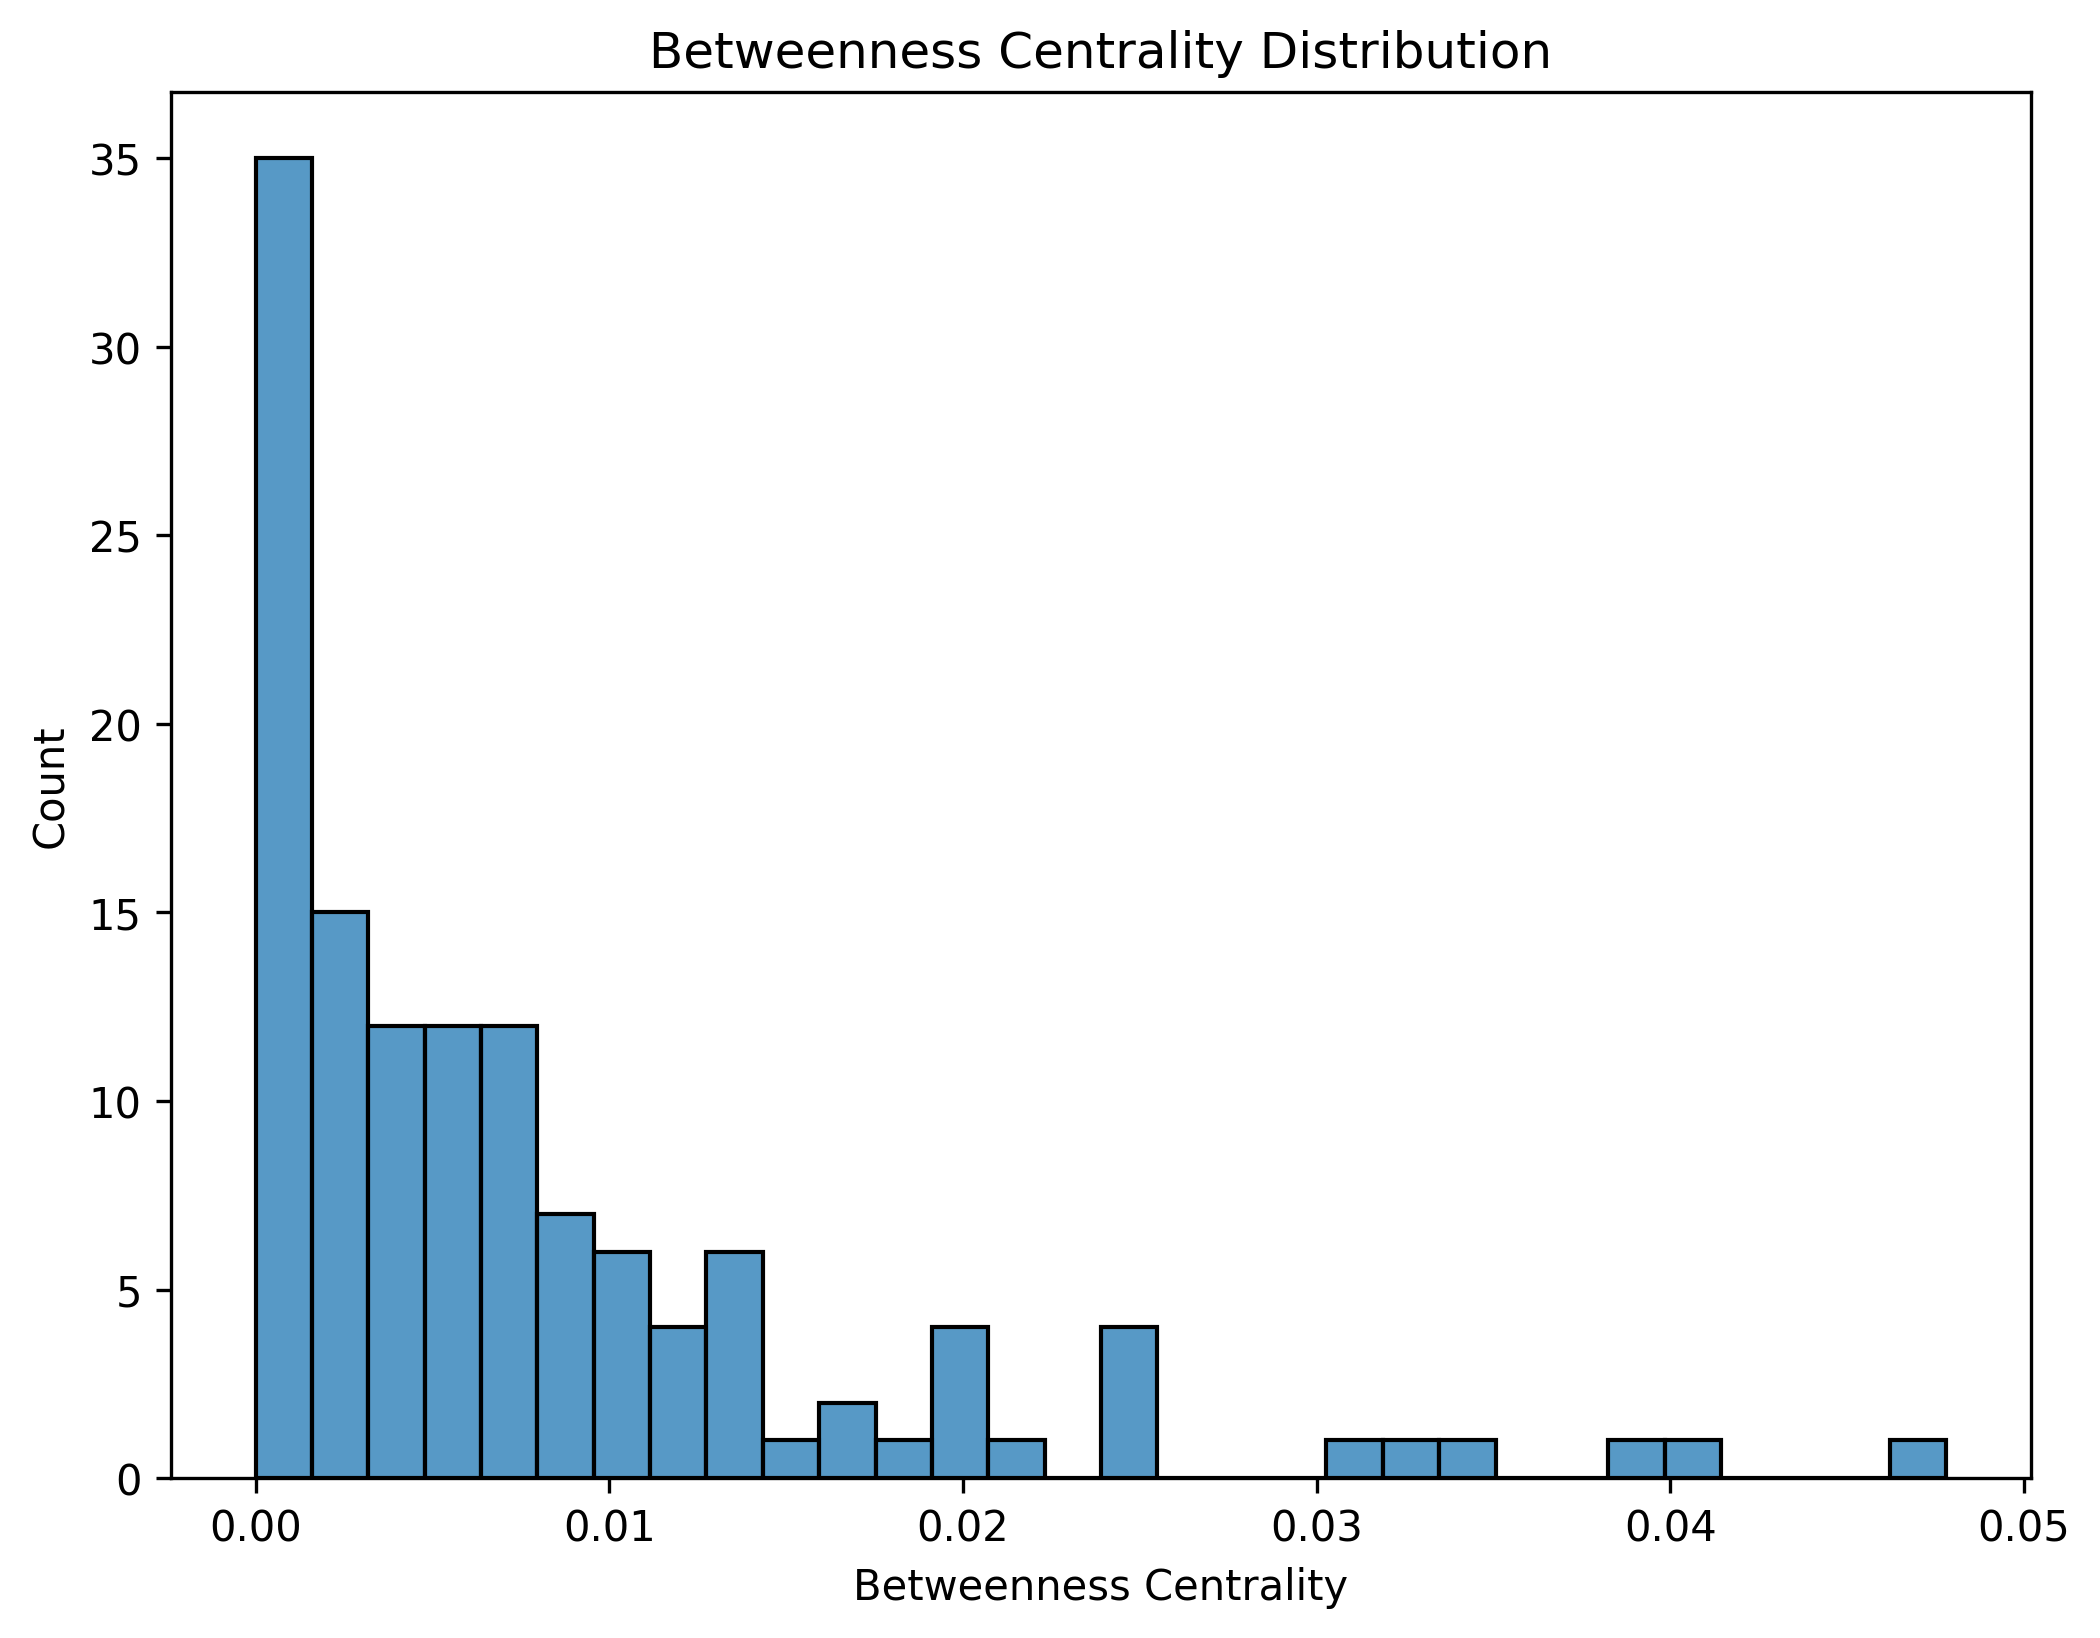
\includegraphics[width=0.8\textwidth]{figures/betweenness_distribution.png}
    \caption{Distribution of betweenness centrality scores across all cities.}
    \label{fig:betweenness_dist}
\end{figure}

The distribution reveals:
\begin{itemize}
    \item Most cities have relatively low betweenness centrality
    \item A small number of cities have significantly higher scores
    \item Clear separation between high and low betweenness cities
\end{itemize}

Figure \ref{fig:top_betweenness} shows the top 10 cities by betweenness centrality:

\begin{figure}[H]
    \centering
    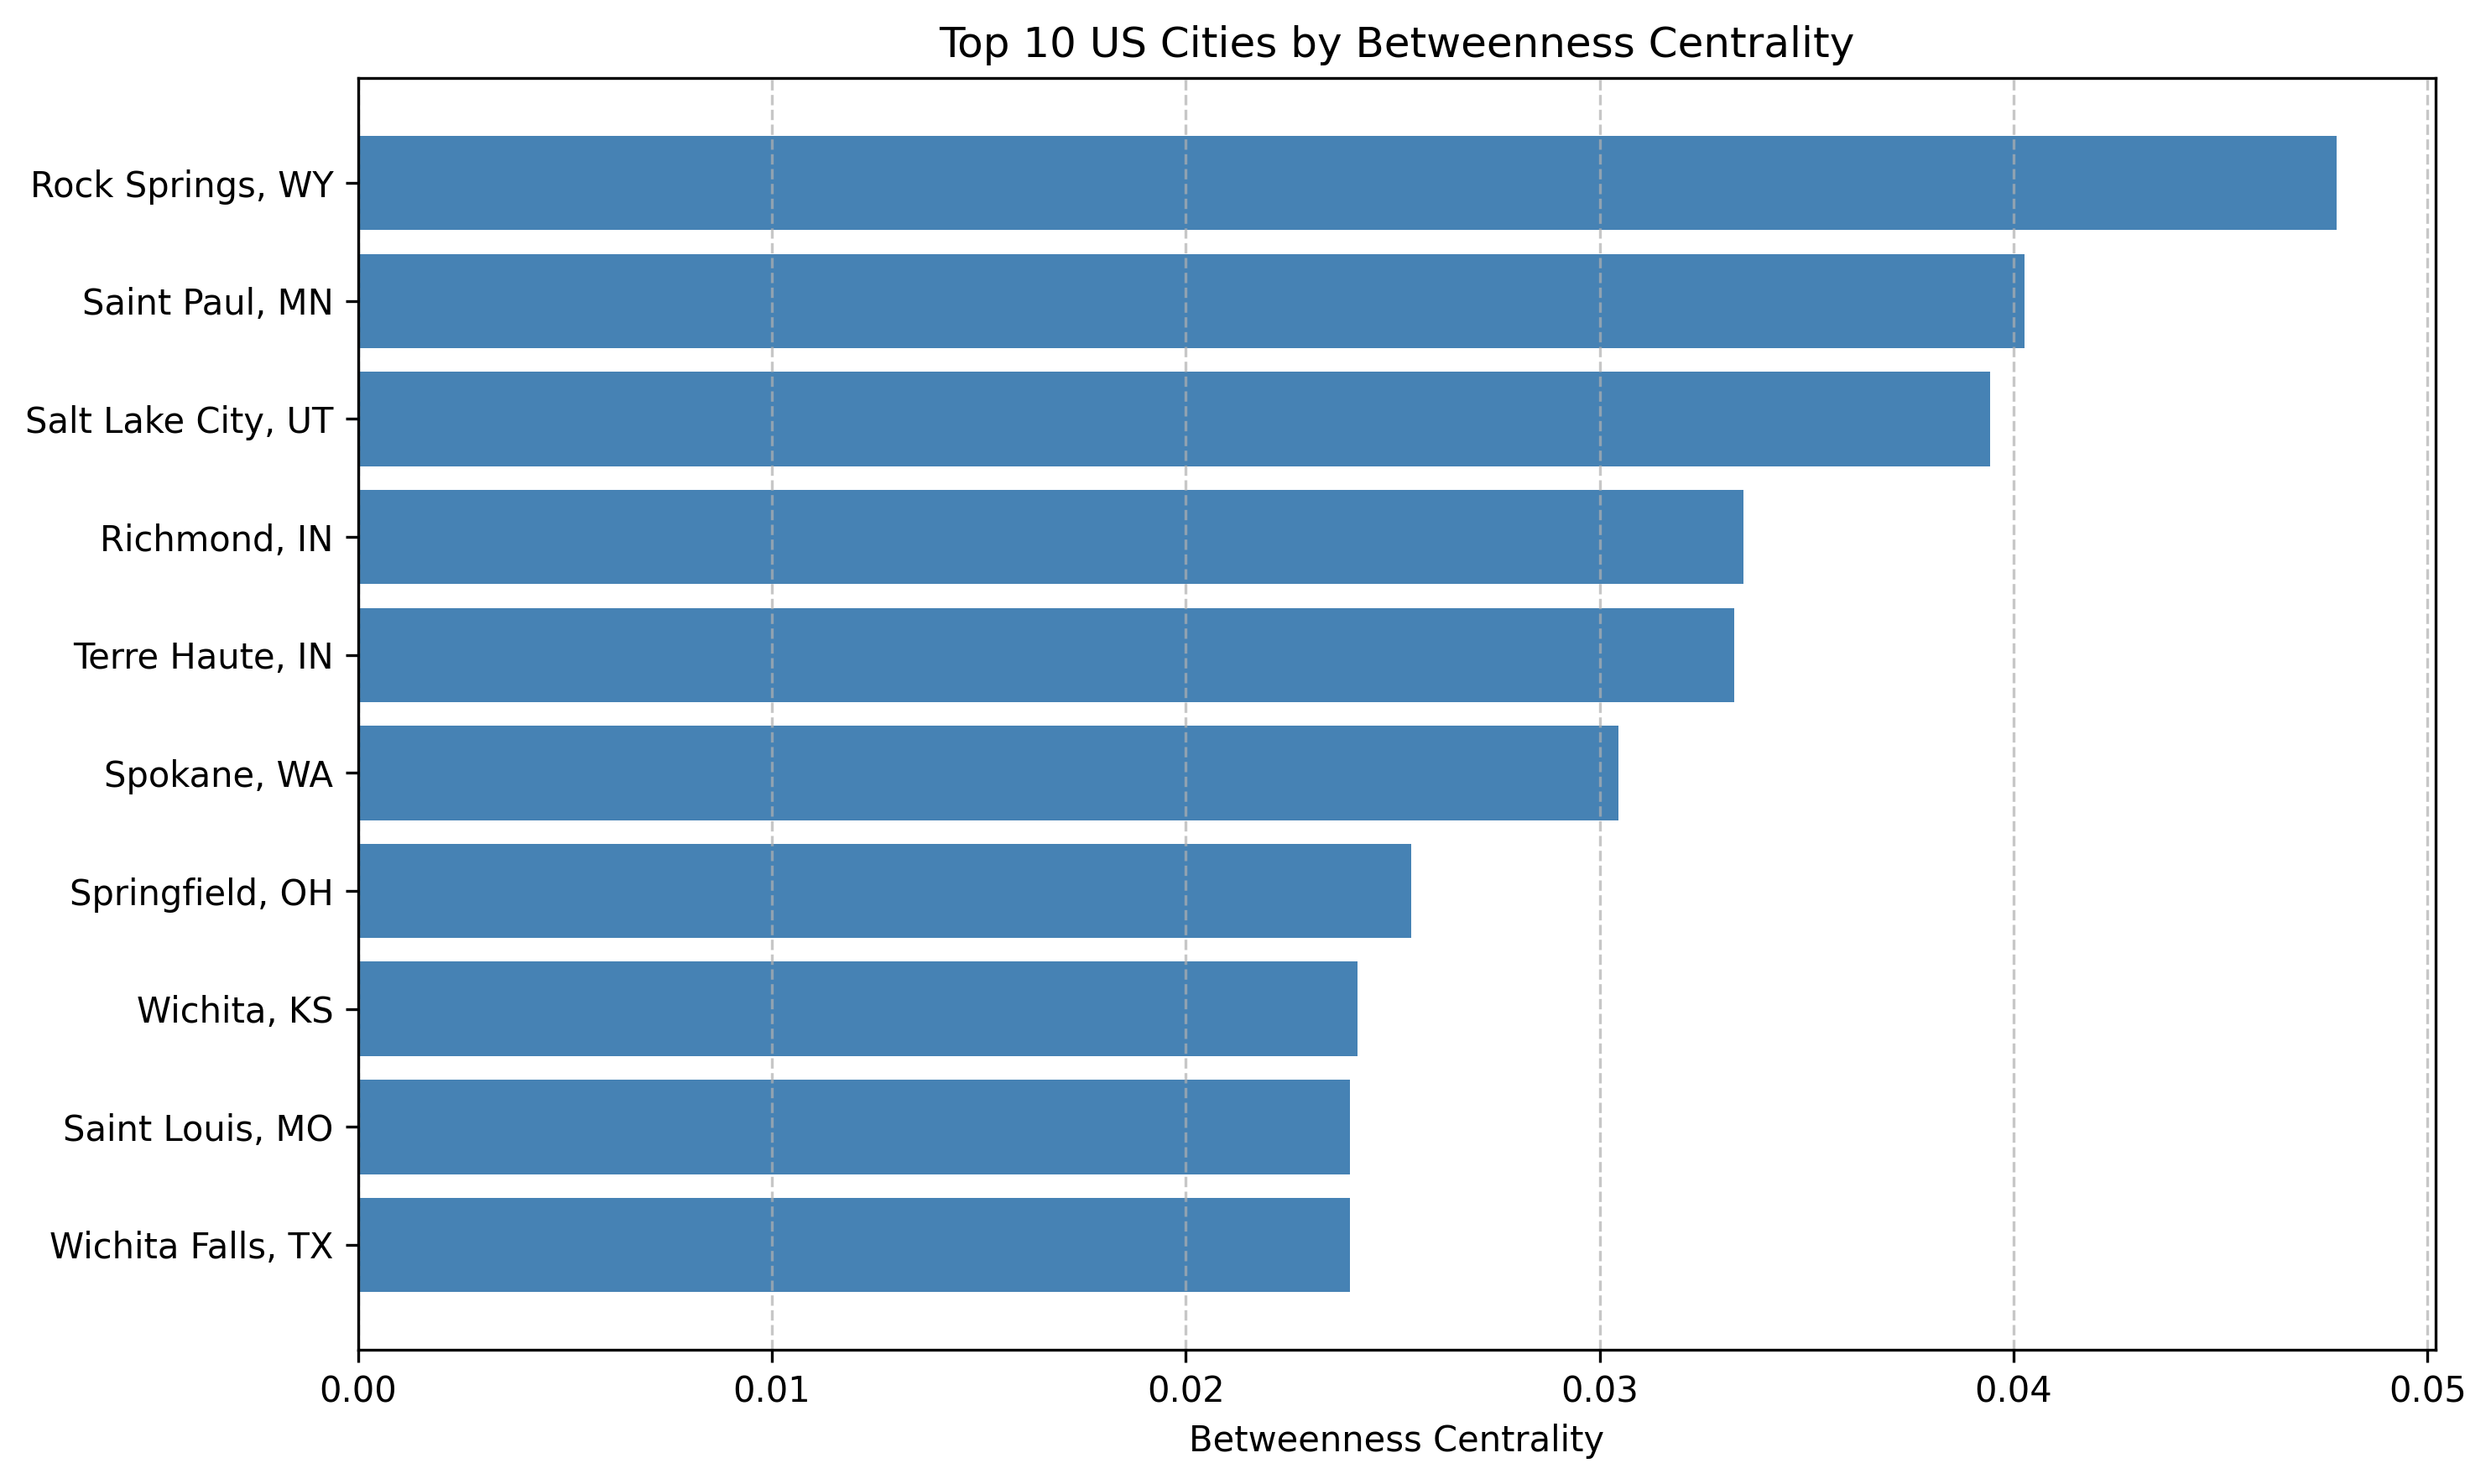
\includegraphics[width=0.8\textwidth]{figures/top_betweenness.png}
    \caption{Top 10 cities by betweenness centrality.}
    \label{fig:top_betweenness}
\end{figure}

Key observations:
\begin{itemize}
    \item Cities in the central United States dominate the top rankings
    \item Clear geographical pattern in high-betweenness cities
    \item Important role of cities in connecting different regions
\end{itemize}

\subsection{Interpretation}
High betweenness centrality indicates cities that:
\begin{itemize}
    \item Serve as important transit points
    \item Connect different regions of the network
    \item Play crucial roles in maintaining network connectivity
\end{itemize}

\section{Closeness Centrality}
\subsection{Definition and Calculation}
Closeness centrality measures how close a node is to all other nodes in the network. It is calculated as:
\begin{equation}
C_C(v) = \frac{1}{\sum_{u \neq v} d(v,u)}
\end{equation}
where $d(v,u)$ is the shortest-path distance between nodes v and u.

\subsection{Top Cities by Closeness Centrality}
The analysis reveals the following top cities:
\begin{enumerate}
    \item Springfield, IL (0.0010)
    \item Saint Louis, MO (0.0010)
    \item Terre Haute, IN (0.0010)
    \item Vincennes, IN (0.0010)
    \item Rockford, IL (0.0010)
\end{enumerate}

Figure \ref{fig:closeness_dist} shows the distribution of closeness centrality scores:

\begin{figure}[H]
    \centering
    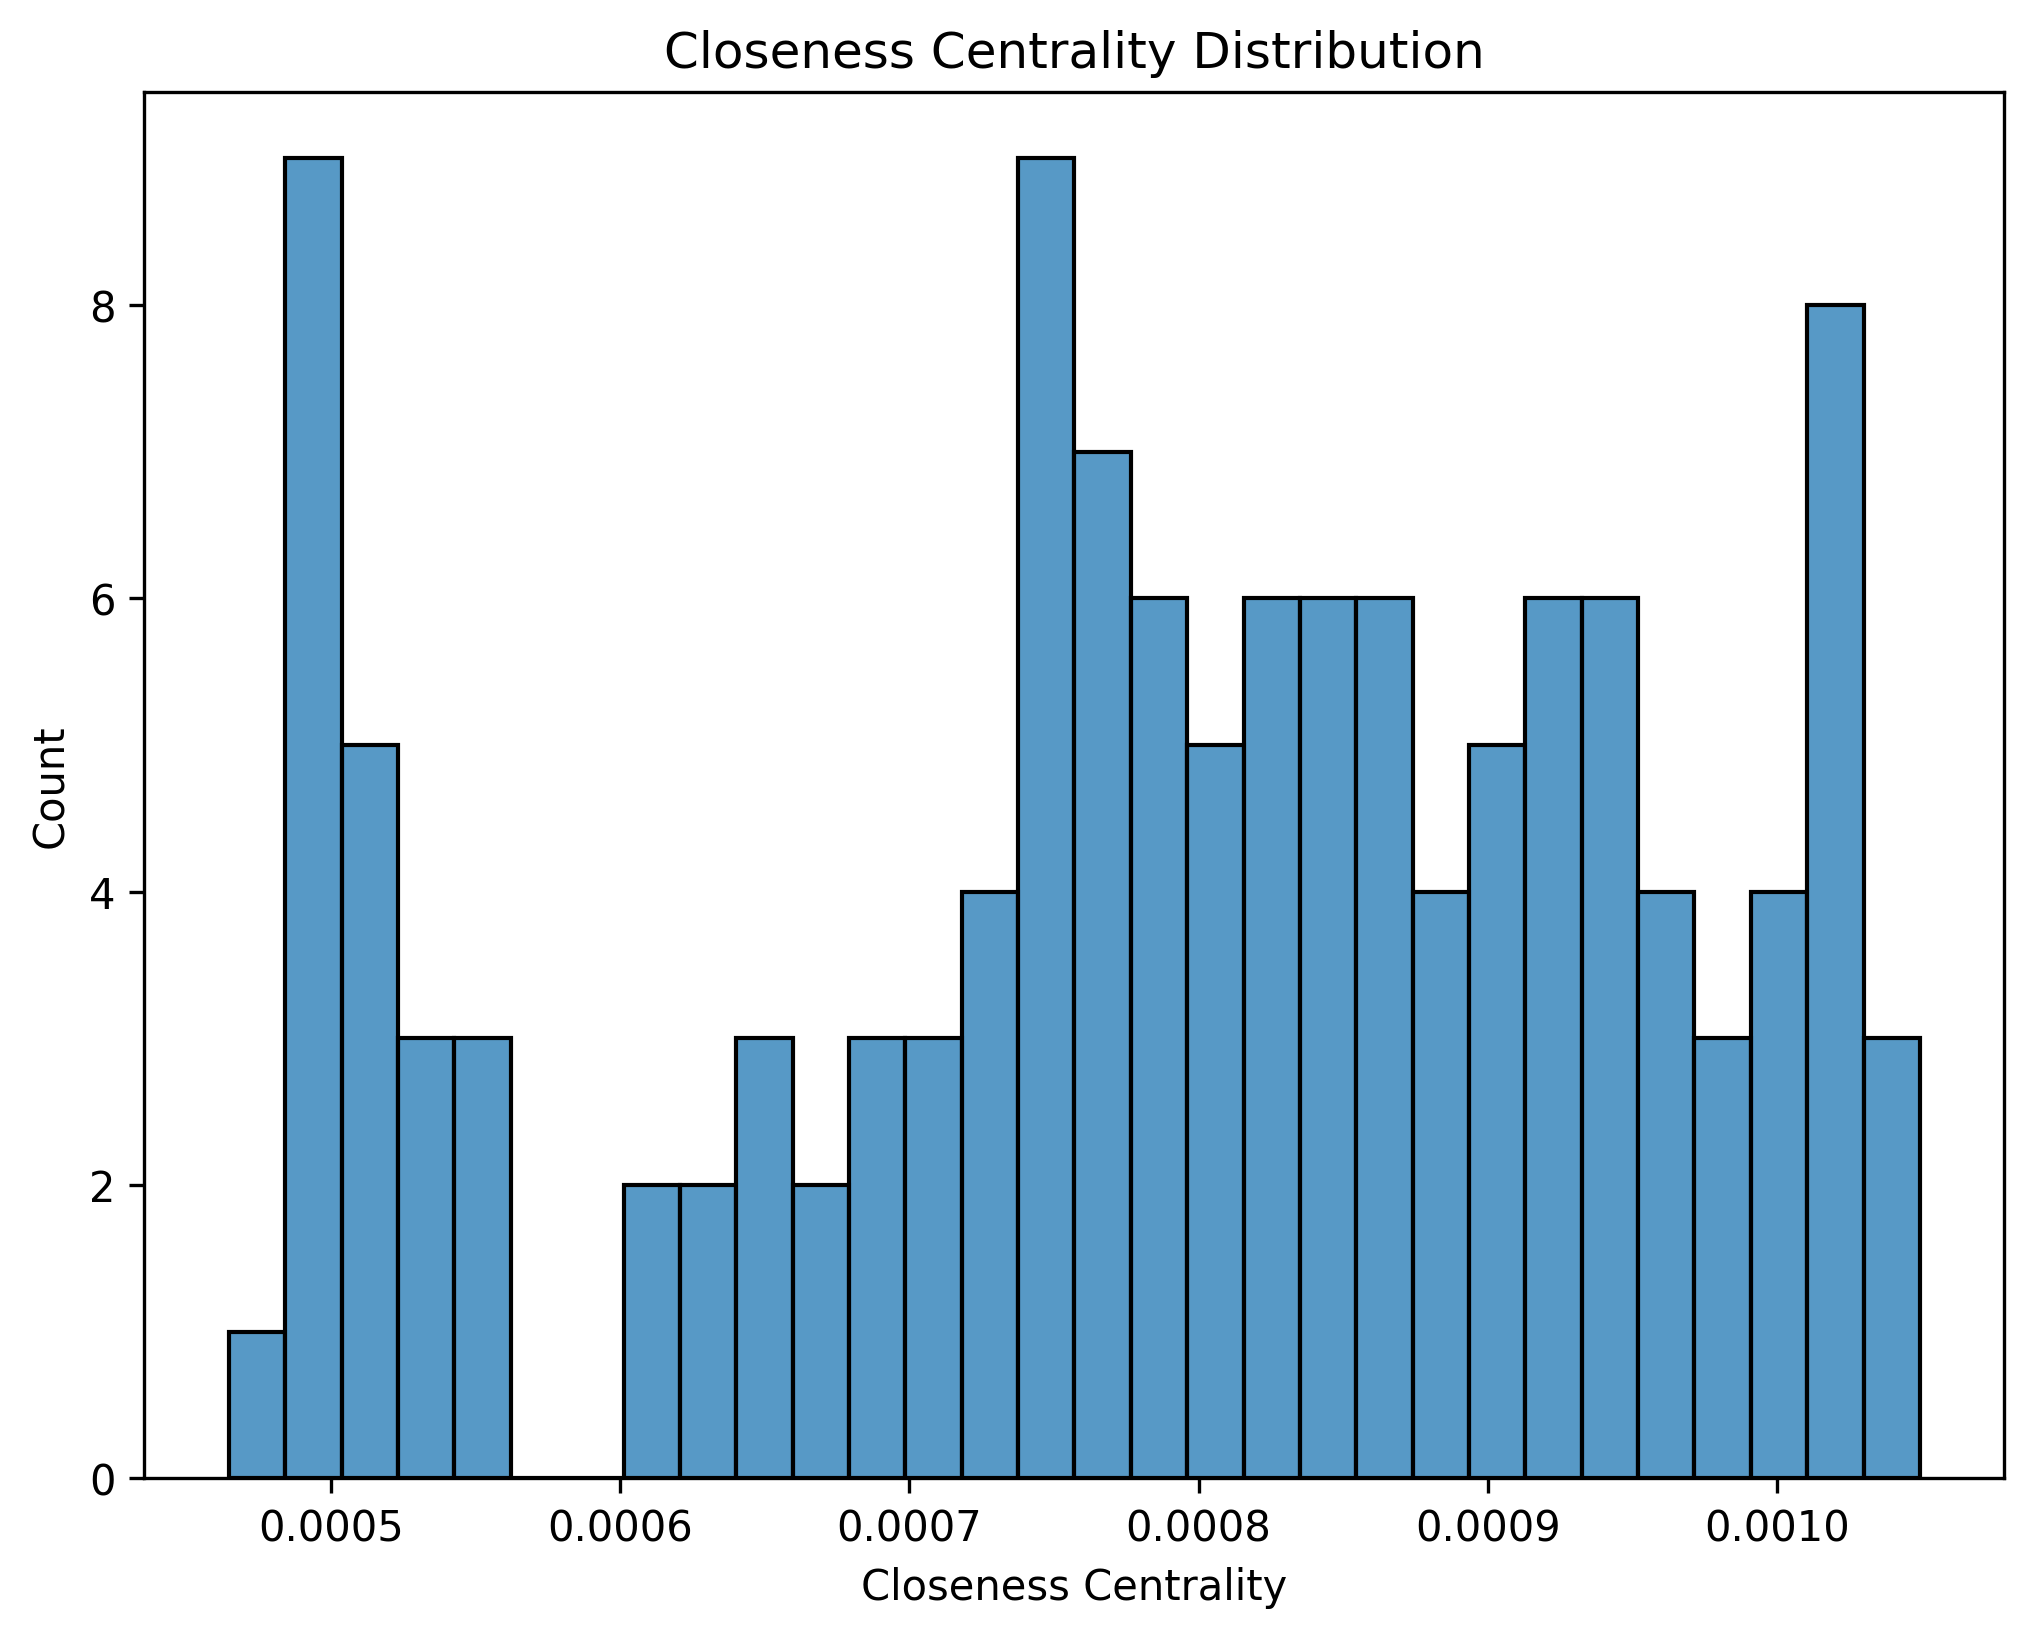
\includegraphics[width=0.8\textwidth]{figures/closeness_distribution.png}
    \caption{Distribution of closeness centrality scores across all cities.}
    \label{fig:closeness_dist}
\end{figure}

The distribution reveals:
\begin{itemize}
    \item Most cities have similar closeness centrality scores
    \item Small variations in scores reflect geographical positioning
    \item Central location leads to higher closeness centrality
\end{itemize}

Figure \ref{fig:top_closeness} shows the top 10 cities by closeness centrality:

\begin{figure}[H]
    \centering
    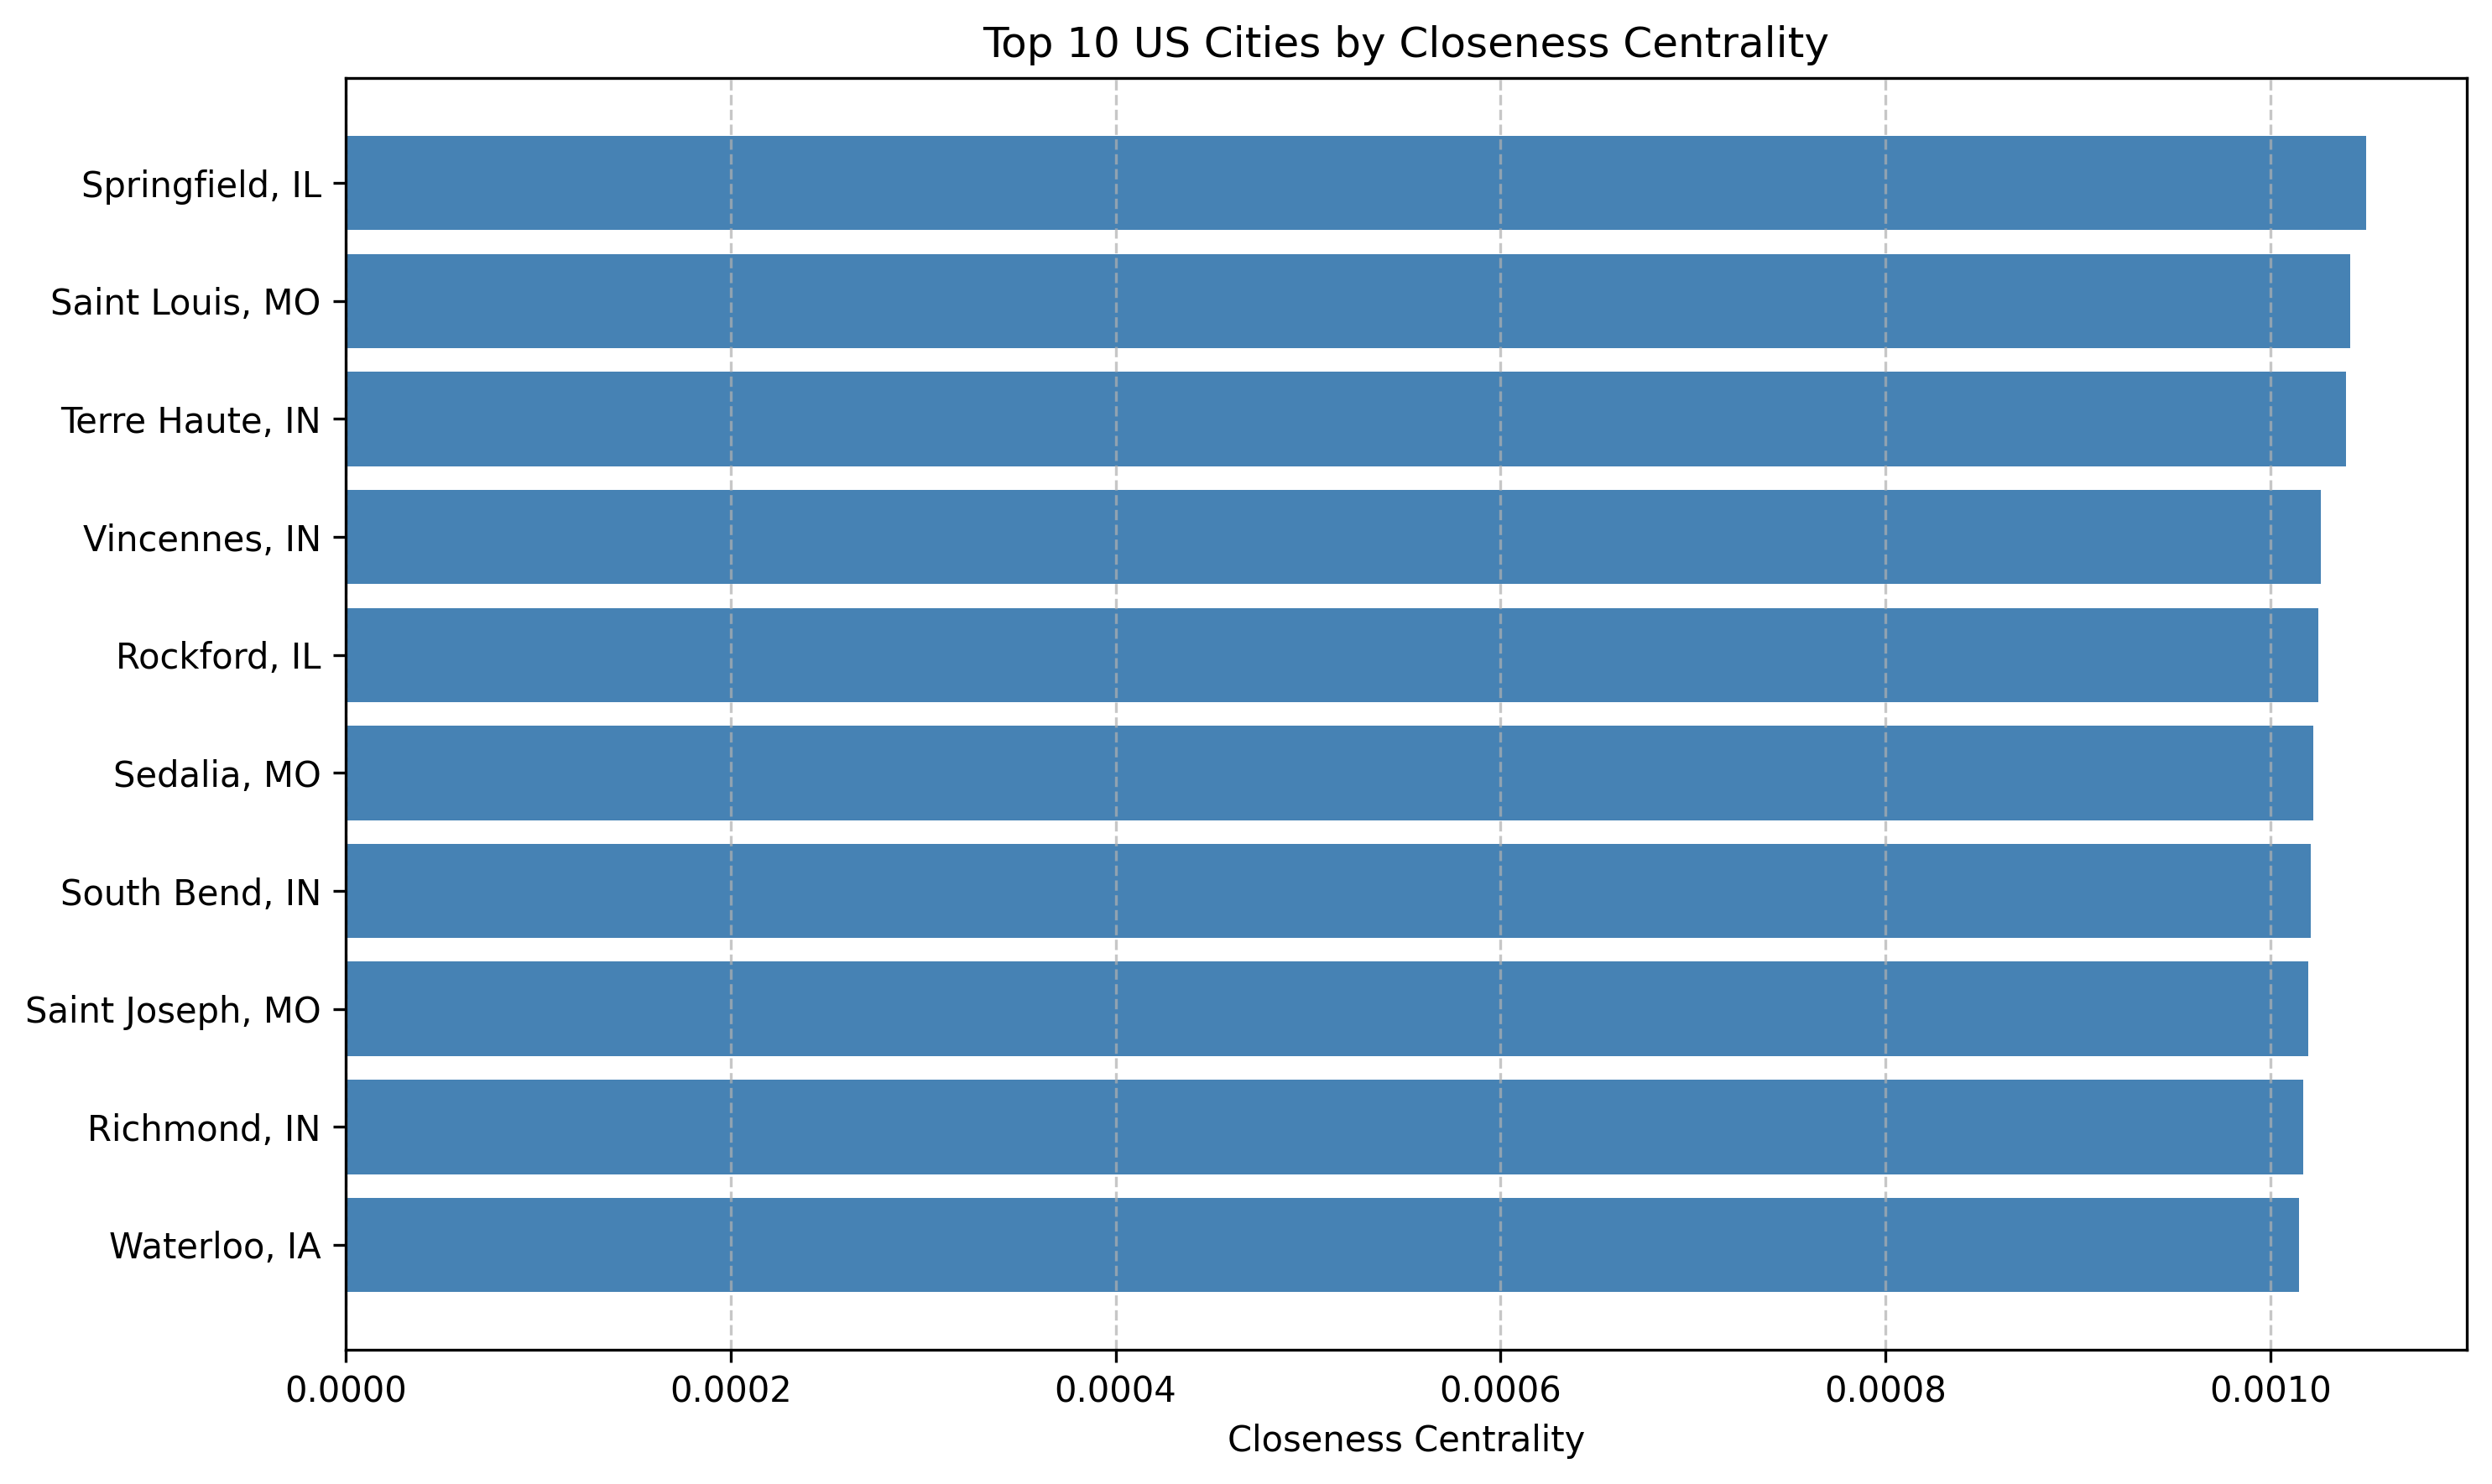
\includegraphics[width=0.8\textwidth]{figures/top_closeness.png}
    \caption{Top 10 cities by closeness centrality.}
    \label{fig:top_closeness}
\end{figure}

Key observations:
\begin{itemize}
    \item Cities in the central United States have highest closeness
    \item Clear geographical pattern in high-closeness cities
    \item Importance of central location for accessibility
\end{itemize}

\subsection{Interpretation}
High closeness centrality indicates cities that:
\begin{itemize}
    \item Are most accessible to other cities
    \item Have the shortest average distance to all other cities
    \item Are centrally located in the network
\end{itemize}


\section{Implications}

The centrality analysis reveals:
\begin{itemize}
    \item Weak correlation between different centrality measures
    \item Different measures capture different aspects of city importance
    \item Need for multiple measures to understand city roles
    \item Central US cities tend to have higher centrality scores
    \item Cities in the Midwest and Great Plains regions show high betweenness
    \item Cities in the central region show high closeness
\end{itemize}


The centrality analysis has several implications:
\begin{itemize}
    \item Transportation planning and infrastructure development
    \item Regional development strategies
    \item Urban network optimization
    \item Understanding of city roles in the national network
\end{itemize}

This comprehensive centrality analysis provides valuable insights into the roles and importance of different cities in the North American urban network. 